\documentclass[t]{beamer}
\usepackage{susu}

\begin{document}
	
	\firstpage
	\justifying
\section{Введение}

	\begin{frame}
		\frametitle{\insertsection} 
		В современном мире остро возникла проблема загрязнения воздуха. Выбросы заводов и автомобилей приводят к повышению температуры воздуха и загрязнению атмосферы химическими соединениями. Решение этой проблемы -- сокращение количества выбросов в атмосферу вредных соединений промышленными предприятиями путем контроля их количества.
	\end{frame}

	\begin{frame}
		\frametitle{Цели и задачи} 
		\textbf{Целью} данной работы является расчет геометрических и физических свойств выбросов предприятий. Для достижения данной цели необходимо решить следующие задачи:
		\begin{enumerate}
			\justifying
			\item исследование существующих методов для контроля выбросов;
			\item исследование современных способов применения оптических и тепловых снимков;
			\item разработка алгоритма для сегментации факела выбросов с использованием тепловых и оптических снимков;
		\end{enumerate}
	\end{frame}

\section[Современные методы]{Современные методы контроля выбросов}
	\begin{frame}
		\frametitle{\insertsection} 
		\bfseries Инструментальный метод \normalfont -- осуществление контроля с помощью газоаналитических средств. Особенности этого метода:
		\begin{enumerate}
			\justifying
			\item подходит для работы с организованными источниками;
			\item для реализации данного метода преимущественно используются газоанализаторы;
			\item высокая точность, что является преимуществом;
			\item сложность настройки и эксплуатации, высокая стоимость используемой аппаратуры, что явлеяется недостатком.
		\end{enumerate}
	\end{frame}
	
	\begin{frame}
		\bfseries Расчетный метод \normalfont используется для расчетов рассеивания выбросов от источников выброса загрязняющих атмосферный воздух веществ с помощью формул. Особенности этого метода:
		\begin{enumerate}
			\justifying
			\item менее точный, что является серьезным минусом;
			\item более дешевым в сравнении с инструментальным методом; 
			\item необходимость установки сложной и дорогой аппаратуры все еще есть, что делает этот метод все еще достаточно затратным.
		\end{enumerate}
	\end{frame}

	\begin{frame}
		Решением данной проблемы может являтся использование тепло-видео систем наблюдения. Их преемущества: 
		\begin{enumerate}
			\justifying
			\item большая дешевизна;
			\item относительно высокая точность.
		\end{enumerate}
		\begin{figure}[h!]
			\centering
			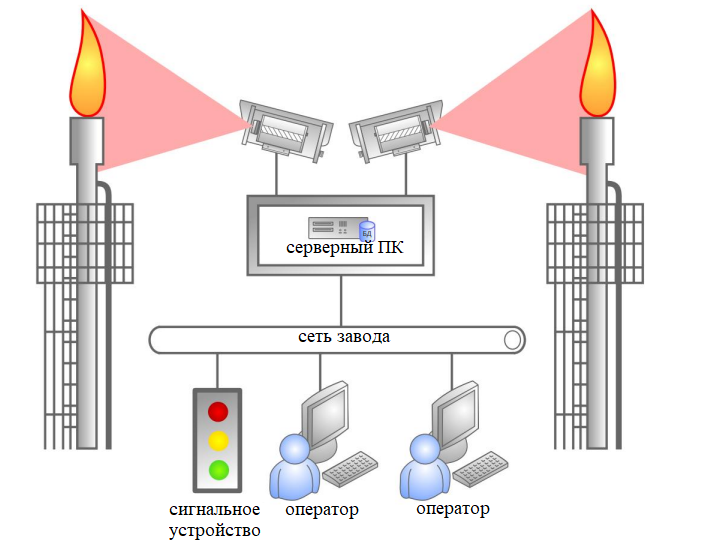
\includegraphics[width = 6cm]{image/controlGasSystem}	
			\caption{Пример использования тепловизоров для сегментации газа}
			\label{fig:controlGasSystem}
		\end{figure}
	\end{frame}

\section{Задача}

	\begin{frame}
		\frametitle{\insertsection} 
		Необходимо востановить целевую функцию
		\vspace*{-0.2cm}
		\begin{equation}
			f: X \rightarrow Z,
			\label{eq:segment_func}
			\vspace*{-0.3cm}
		\end{equation}
	где $X$ -- пары RGB изображений и матриц температур;
	$Y$ - маска где каждый элемент -- принадлежность пикселя дыму.
	\begin{figure}[ht!]
		\begin{subfigure}{.23\textwidth}
			\centering
			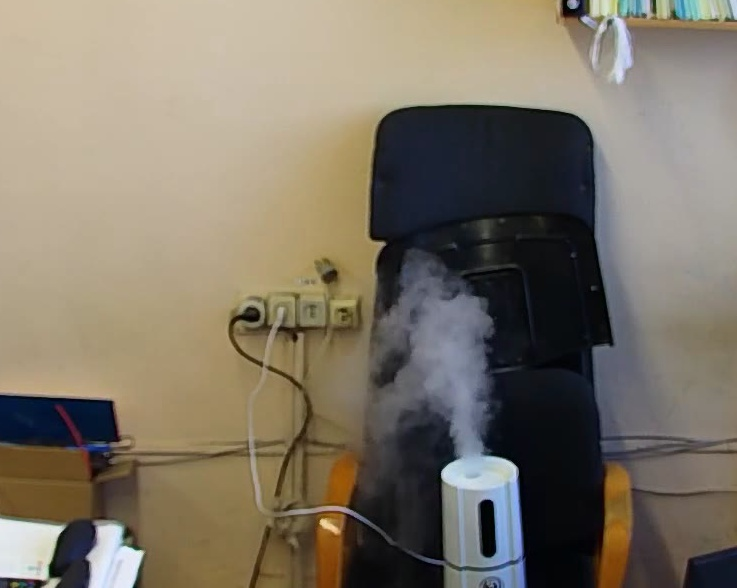
\includegraphics[width = \textwidth]{image/opt_examp}
			\caption{}
		\end{subfigure}
		\begin{subfigure}{.23\textwidth}
			\centering
			
\includegraphics[width = \textwidth]{image/tep_examp}
			\caption{}
		\end{subfigure}
		\begin{subfigure}{.23\textwidth}
			\centering
			
\includegraphics[width = \textwidth]{image/mask}
			\caption{}
		\end{subfigure}
		\centering
		\caption{Примеры полученых изображений, где (a) RGB изображение;(б) матрица температур; (г) полученная маска}
		\label{fig:Examples}
	\end{figure}
	\end{frame}

\section{Подготовка данных}

	\begin{frame}
		\frametitle{\insertsection} 
		Для решения поставленной задачи необходимо разработать алгоритм взаимодействия с тепловизором и научиться получать данные для последующей обработки. Подготовку данных можно разделить на три этапа:
		\begin{enumerate}
			\item работа с тепловизором;
			\item преобразование цветовой карты;
			\item наложение карты абсолютных температур на оптические снимки.
		\end{enumerate}
	\end{frame}

	\begin{frame}
		\textbf{Работа с тепловизором.}
		
		Было решено записывать поток оптически и тепловых снимков с частотой 20 Ггц и максимальную и минимальную температуры с частотой в 1 Ггц. Оптические и тепловые снимки записываются в формате YUV.
		\begin{figure}[ht!]
			\begin{subfigure}{.45\textwidth}
				\centering
				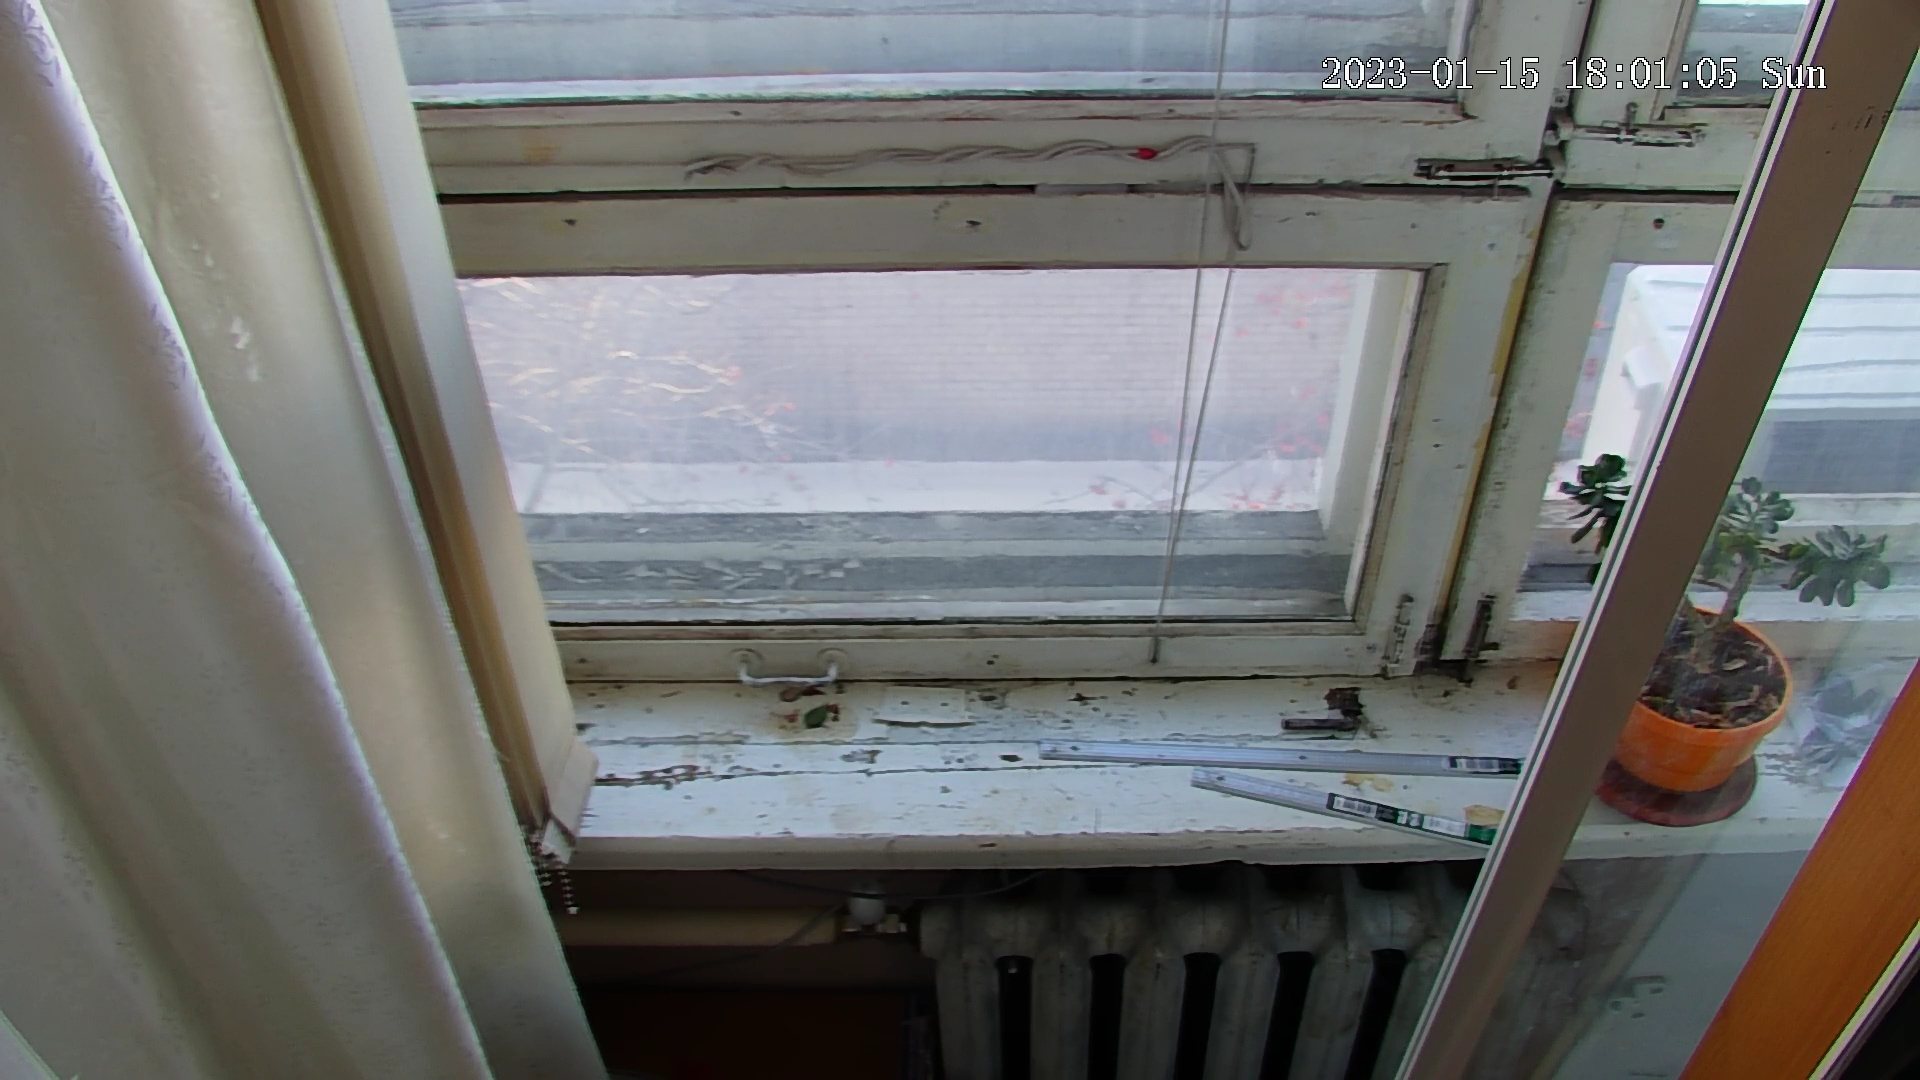
\includegraphics[width = 3cm]{image/chapter_2/opt_example}
				\caption{}
			\end{subfigure}
			\begin{subfigure}{.45\textwidth}
				\centering
				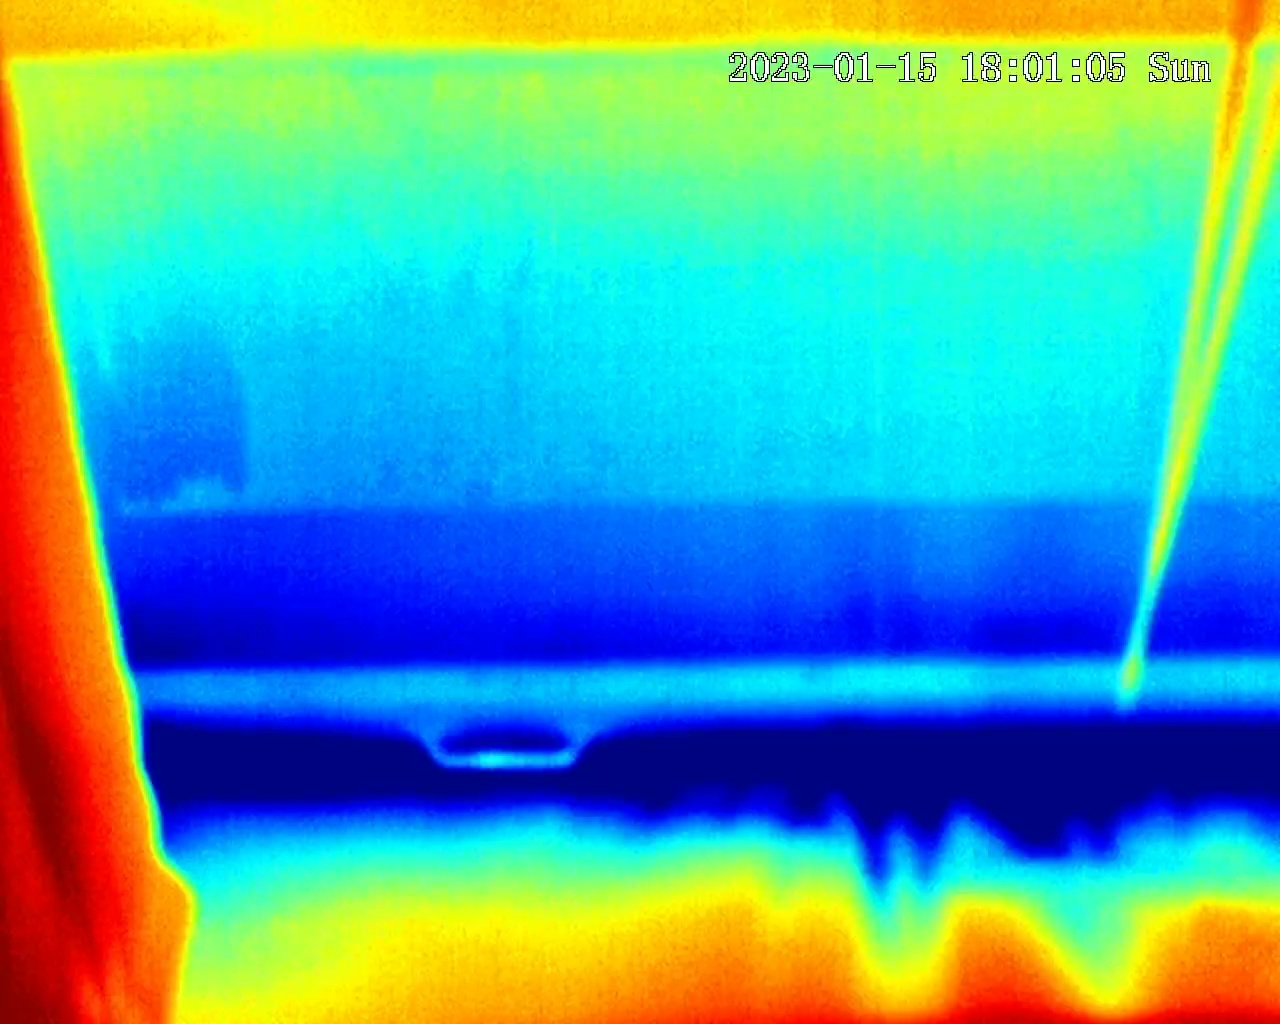
\includegraphics[width = 3cm]{image/chapter_2/tep_example}
				\caption{}
			\end{subfigure}
			\centering
			\caption{Примеры полученых изображений, где (a) оптический снимок; (б) тепловой снимок}
			\label{fig:Examples}
		\end{figure}
	\end{frame}

	\begin{frame}
		\begin{figure}[h!]
			\centering
			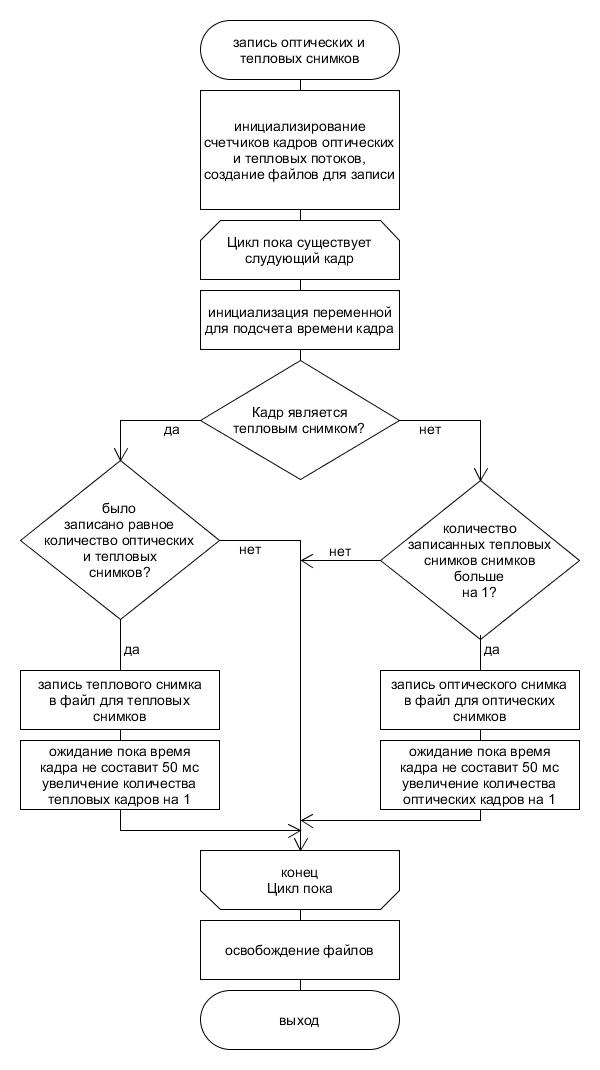
\includegraphics[width = 0.34\textwidth]{image/chapter_2/loaddata}	
			\caption{Алгоритм сохранения снимков}
			\label{fig:loaddata}
		\end{figure}
	\end{frame}

	\begin{frame}
		\bfseries Преобразование цветовой карты. \normalfont
		На рисунке~\ref{fig:Examples} видно, что тепловые снимки записываются с использованием цветовой карты.  В нашем случае была применена цветовая карта <<JET>>. Необходимо востановить функцию преобразования к оттенкам серого, классифицировав цвета RGB.
		\begin{figure}[ht!]
			\begin{subfigure}{.45\textwidth}
				\centering
				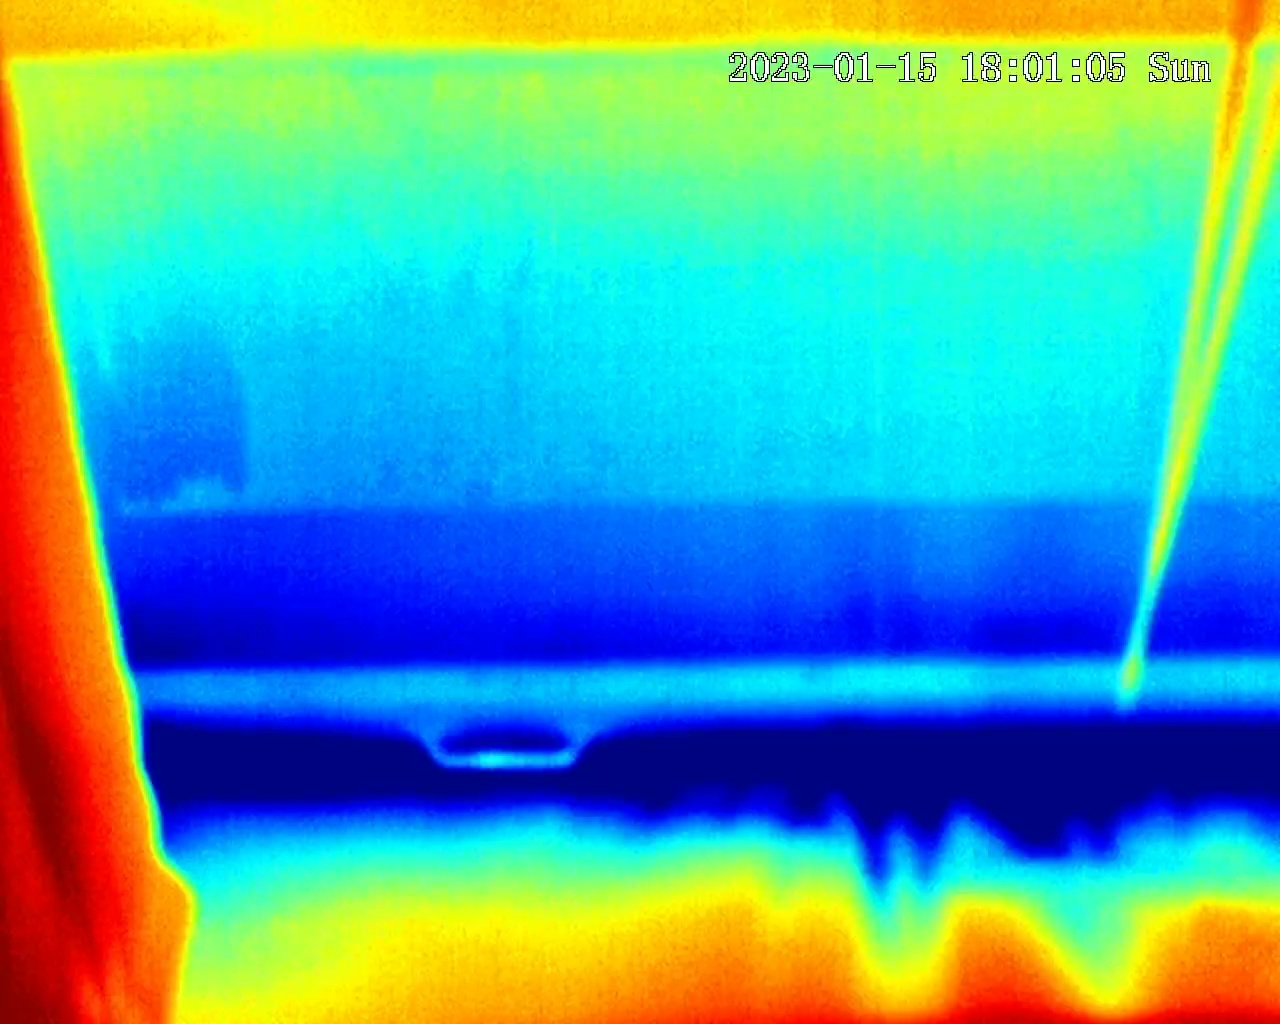
\includegraphics[width = 4cm]{image/chapter_2/tep_example}
				\caption{}
			\end{subfigure}
			\begin{subfigure}{.45\textwidth}
				\centering
				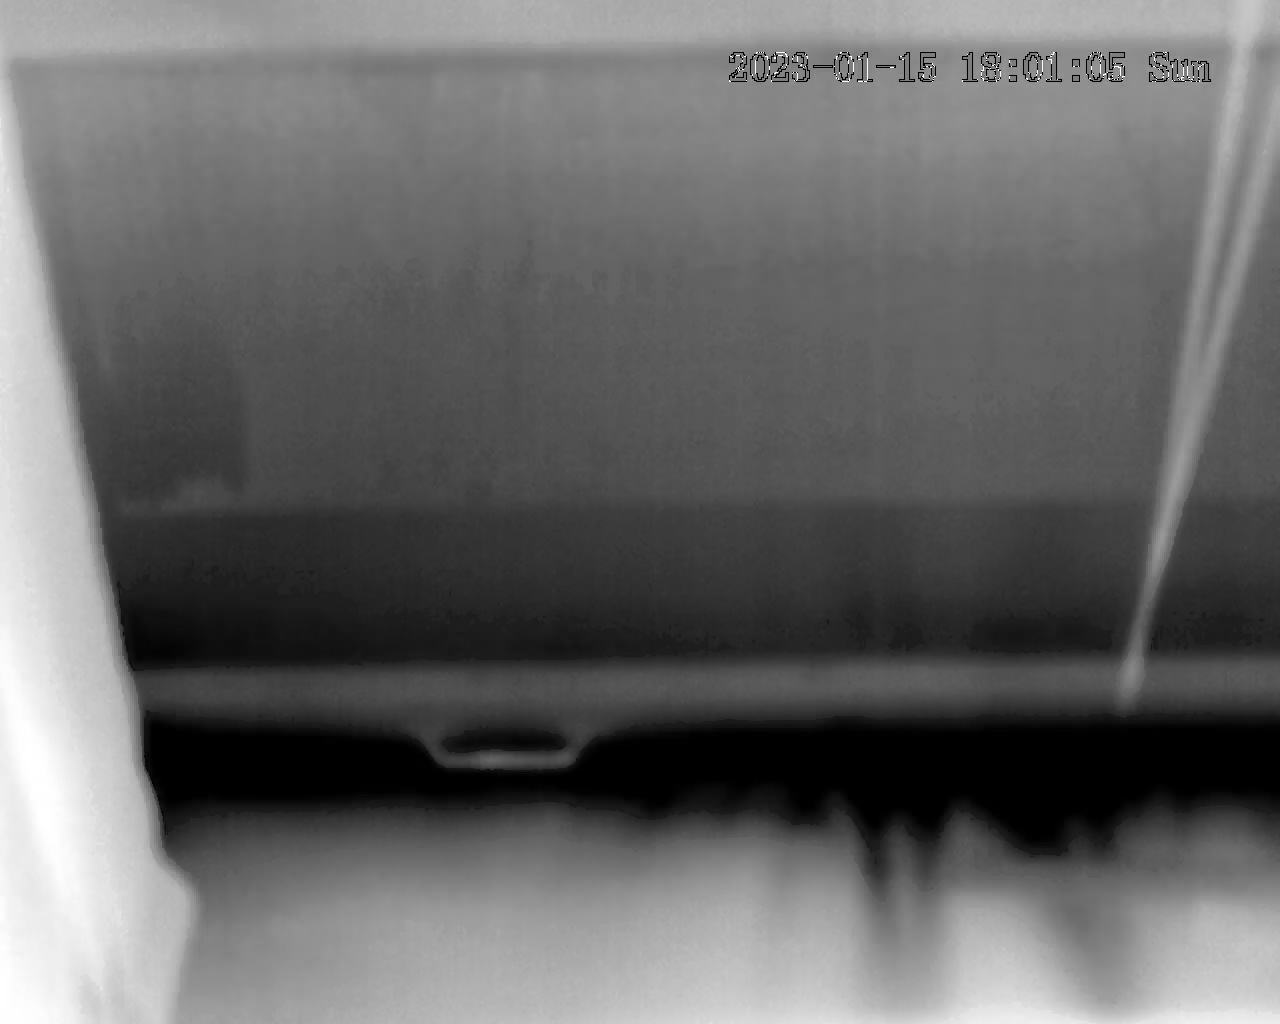
\includegraphics[width = 4cm]{image/chapter_2/gray_tep_example}
				\caption{}
			\end{subfigure}
			\centering
			\caption{Примеры преобразования цветовой карты, где (a) до; (б) после}
			\label{fig:ResKNN}
		\end{figure}
	\end{frame}

	\begin{frame}
		\textbf{Модель <<FlannBasedMatcher>>}
		
		Эта модель решает задачу классификации и работает на основе метода $k$-ближайших соседей, оптированного с помощью структуры данных <<$k$-мерное дерево>>.
		\begin{figure}[h!]
			\centering
			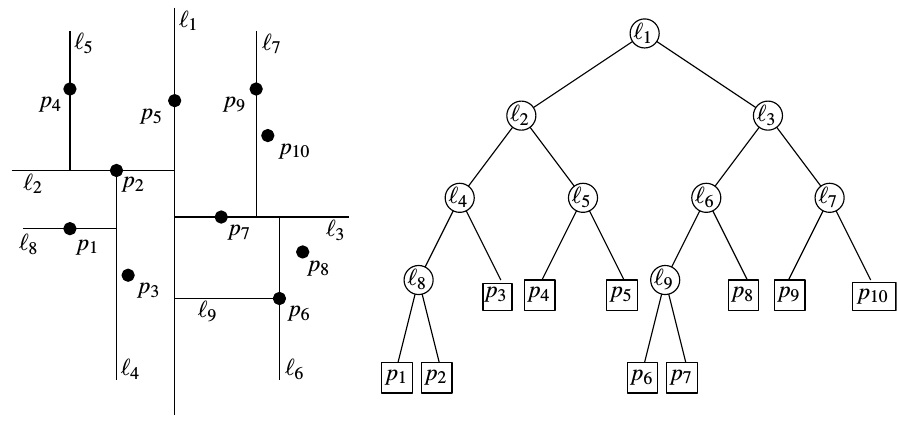
\includegraphics[width = 6cm]{image/chapter_2/kdtreeexample}	
			\caption{Пример построения k-мерного дерева}
			\label{fig:kdtreeexample}
		\end{figure}
	\end{frame}
	
	\begin{frame}
		
		\begin{figure}[ht!]
			\begin{subfigure}{.31\textwidth}
				\centering
				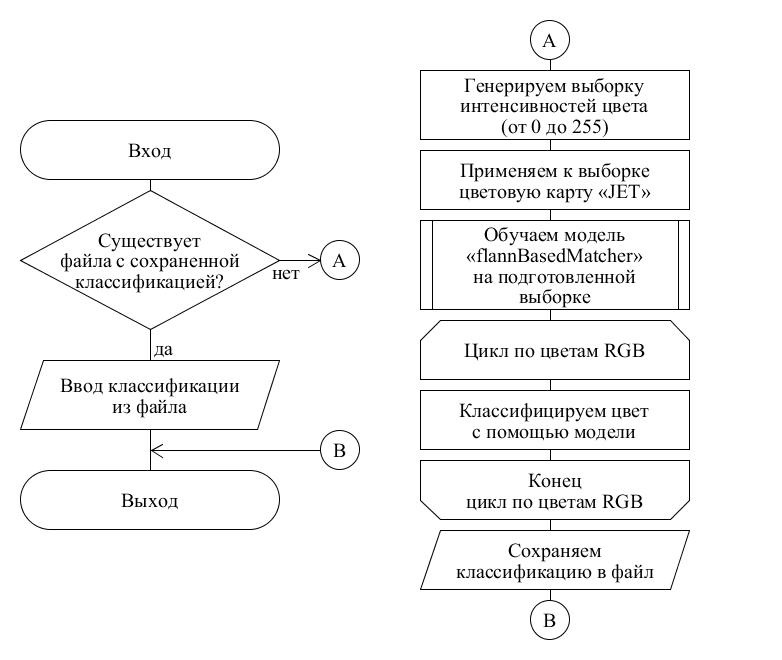
\includegraphics[width = \textwidth]{image/chapter_2/colorclassification}
				\caption{}
			\end{subfigure}
			\begin{subfigure}{.17\textwidth}
				\centering
				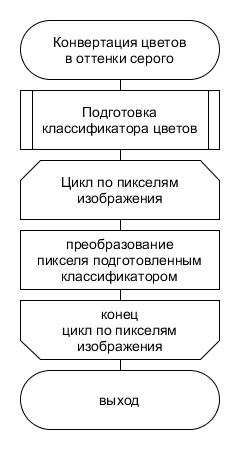
\includegraphics[width = \textwidth]{image/chapter_2/colorclassification2}
				\caption{}
			\end{subfigure}
			\centering
			\caption{Алгоритмы преобразования цветов, где (а) алгоритм подготовки классификатора цветов; (б) алгоритм преобразования}
			\label{fig:Examples}
		\end{figure}
		
	\end{frame}

	\begin{frame}
		Для оценки точности была введена метрика, отражающая среднюю относительную разницу интенсивности пикселя:
		\begin{equation*}
			Acc = 1 - \frac{\sum\limits_{i=1}^h \sum\limits_{j=1}^w |P^{true}_{ij} - P^{conv}_{ij}|}{255wh},
			\label{eq:flanaccuracy}
		\end{equation*}
		где $w$ и $h$ -- размеры кадра. $P^{true}$ и $P^{conv}$ - некоторое изображение в оттенках серого и то же самое изображение, но с наложеной цветовой картой, сжатое с помощью JPEG и обработанное алгоритмом преобразования. В результате была получена точность 0,995777.
	\end{frame}

	\begin{frame}
		
		\begin{figure}[h!]
			\centering
			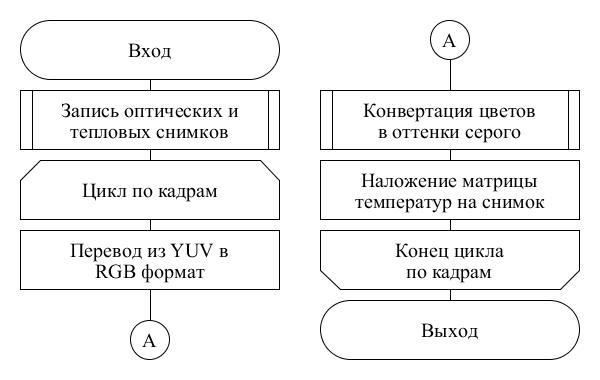
\includegraphics[width = 0.23\textwidth]{image/chapter_2/fullprepare}	
			\caption{Алгоритм подготовки данных}
			\label{fig:fullprepare}
		\end{figure}
		
	\end{frame}

\section{Результаты}

	\begin{frame}
		На данный момент реализована сегментация по методу отсечения по пороговому значению. Порогом является медианная абсолютная температура.
		\begin{figure}[h!]
			\centering
			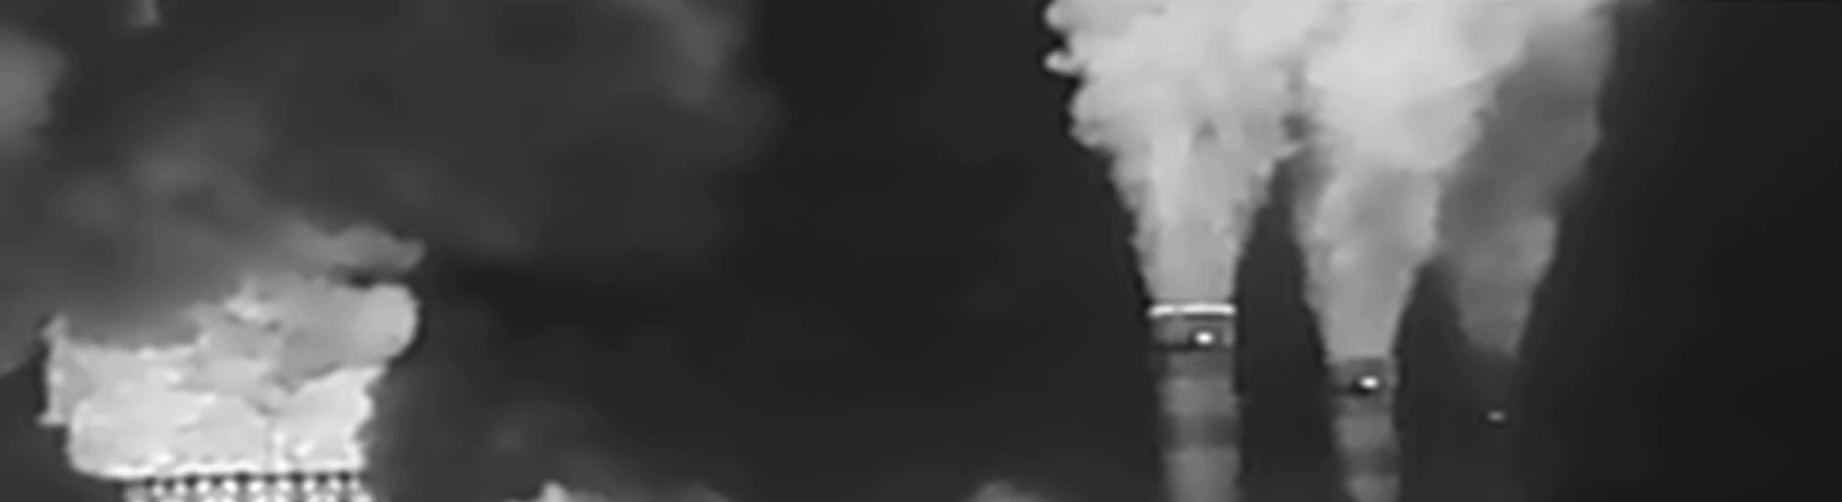
\includegraphics[width = 7cm]{image/img}	
			\caption{Изображение в оттенках серого}
			\label{fig:segbef}
		\end{figure}
		\begin{figure}[h!]
			\centering
			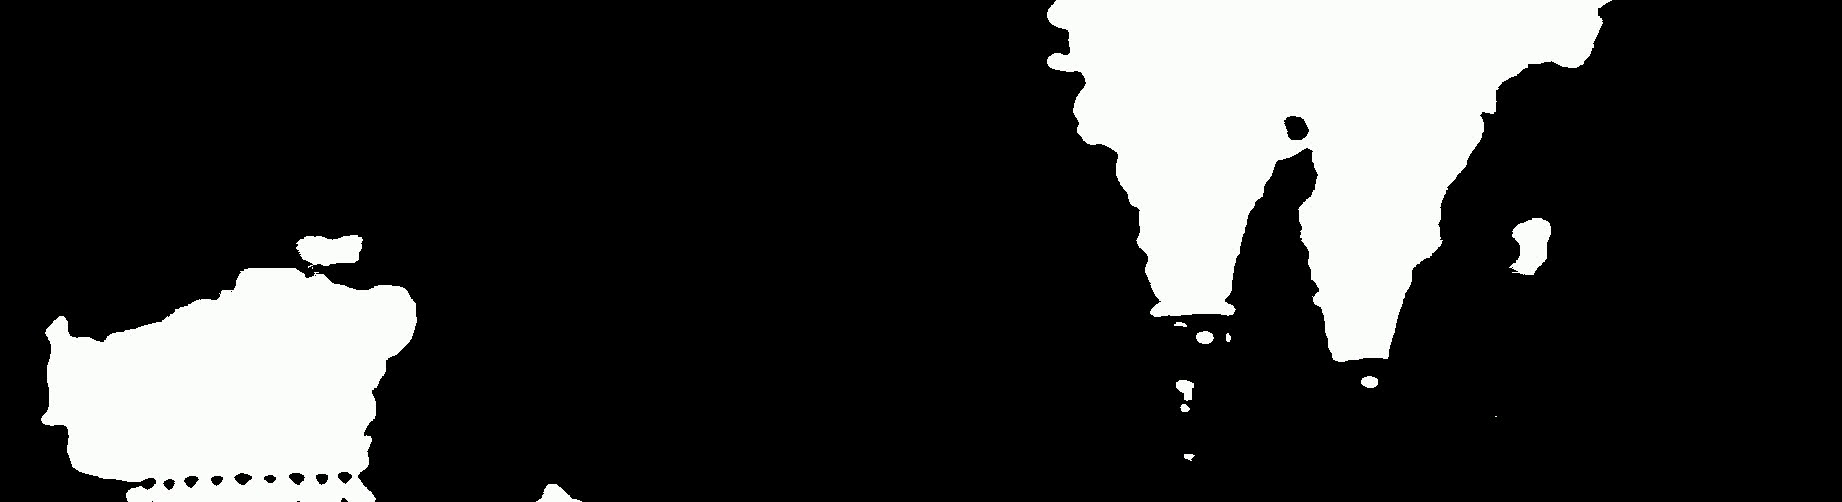
\includegraphics[width = 7cm]{image/seg}	
			\caption{Маска после сегментации}
			\label{fig:segaft}
		\end{figure}
	\end{frame}
	\begin{frame}
	\begin{center}
		\vspace{3cm}
		\Huge{Спасибо за внимание!}
	\end{center}
	\end{frame}

\end{document}
